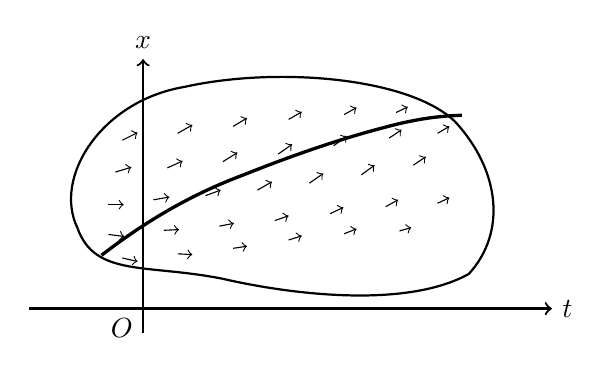
\begin{tikzpicture}[x=0.88cm,y=0.88cm,thick]
  \draw[thick] (-3.1,-0.38) .. controls (-3.45,0.35) and (-2.75,1.45) .. (-1.55,1.65)
    .. controls (-0.2,1.95) and (1.7,1.78) .. (2.35,1.15)
    .. controls (3.0,0.45) and (3.1,-0.45) .. (2.55,-1.05)
    .. controls (1.65,-1.55) and (0.0,-1.35) .. (-1.0,-1.12)
    .. controls (-2.1,-0.9) and (-2.85,-1.1) .. (-3.1,-0.38);
  \draw[->] (-3.8,-1.55)--(3.75,-1.55) node[right] {$t$};
  \draw[->] (-2.15,-1.9)--(-2.15,2.05) node[above] {$x$};
  \node[below left] at (-2.15,-1.55) {$O$};
  % A sampled direction field; each small segment has slope depending on t and x.
  \foreach \x/\y/\dx/\dy in {
  -2.65/-0.05/0.22/0.00,-2.0/0.02/0.23/0.04,-1.25/0.08/0.22/0.08,-0.5/0.16/0.21/0.12,0.25/0.26/0.20/0.14,1.0/0.38/0.19/0.14,1.75/0.52/0.18/0.12,
  -2.55/0.42/0.23/0.07,-1.8/0.48/0.22/0.10,-1.0/0.57/0.21/0.13,-0.2/0.68/0.20/0.14,0.6/0.80/0.19/0.14,1.4/0.91/0.18/0.12,2.1/0.98/0.17/0.10,
  -2.45/0.88/0.22/0.11,-1.65/0.98/0.21/0.12,-0.85/1.08/0.20/0.12,-0.05/1.18/0.19/0.11,0.75/1.25/0.18/0.10,1.5/1.28/0.17/0.08,
  -2.65/-0.48/0.23/-0.03,-1.85/-0.42/0.22/0.01,-1.05/-0.36/0.21/0.04,-0.25/-0.28/0.20/0.07,0.55/-0.18/0.19/0.09,1.35/-0.08/0.18/0.10,2.1/-0.03/0.17/0.08,
  -2.45/-0.82/0.22/-0.05,-1.65/-0.76/0.21/-0.01,-0.85/-0.68/0.20/0.03,-0.05/-0.56/0.19/0.06,0.75/-0.47/0.18/0.07,1.55/-0.43/0.17/0.05}
    {\draw[->,thin] (\x,\y)--++(\dx,\dy);}
  \draw[very thick] (-2.75,-0.78) .. controls (-2.1,-0.28) and (-1.45,0.1) .. (-0.7,0.38)
    .. controls (0.1,0.7) and (0.85,0.95) .. (1.55,1.12)
    .. controls (1.9,1.2) and (2.15,1.23) .. (2.45,1.24);
\end{tikzpicture}
